\subsection{Scan periods with spurious signal uncertainties included}
\label{sec:scan_periods_sys}
%%% show significance plot
%%% show fit uncertainties
The significance of injected signals is studied as a function of probing
periods using signal-injected toys. We performed this study using four
types of SME signal shapes, and the injected maximum signal amplitude
for each type of signal is 5\%.  The injected SME signal shapes are
$d_{u}^{X,Z}$, $d_{u}^{Y,Z}$, $d_{u}^{XX-YY}$, $d_{u}^{X,Y}$.

The top left plot in Figure~\ref{fig:scan_period_toy_Sys_combined_fit}
shows the canned significance without systematic included in the fit. As we expected, a huge spike appeared when
the probing period was equal to the sidereal period (23:56:04) because
the signal is injected in the sidereal period.
The top right plot shows the significance with systematic included 
in the fit. The significance is reduced when we add systematics. 
Profiled $\chi^{2}$ fit with systematics does not change the value
of parameters obtained from the fit, as shown in the bottom left plot.
The main contribution of the systematics is in the fit uncertainties. 
The bottom right plot shows the ratio of the fit uncertainties 
with/without systematic inclusion in the fit. The fit uncertainties
are increased; for example, 12.5\% increased in $d_{u}^{X,Z}$ signal shape. 
The impact of a systematic mainly depends on the input size. The corresponding spurious signal systematic are listed in the table~\ref{table:real_data_scrambled_Generic_combined_fit}



\begin{figure}[!ht]
\centering
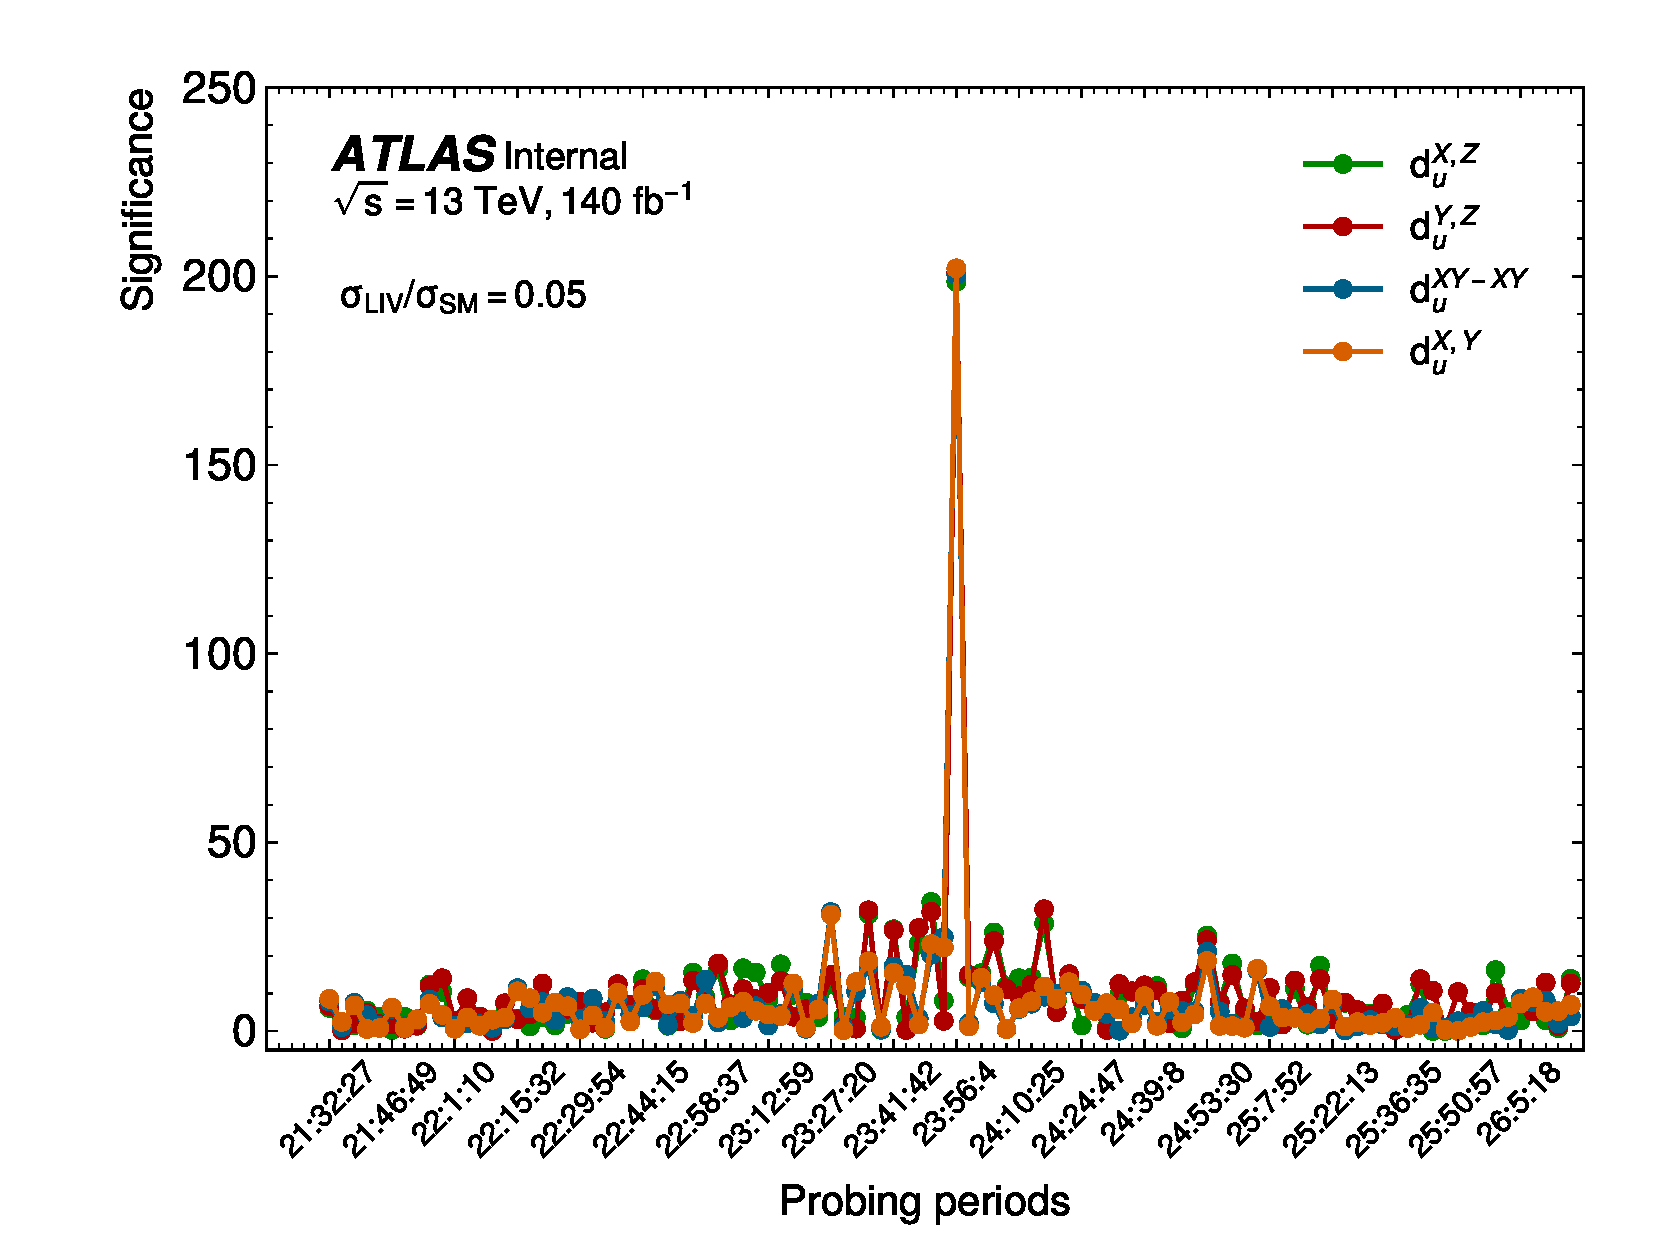
\includegraphics[width=0.45\textwidth]{figs/partially_unblinded_results/scan_periods/scan_significance_toys}
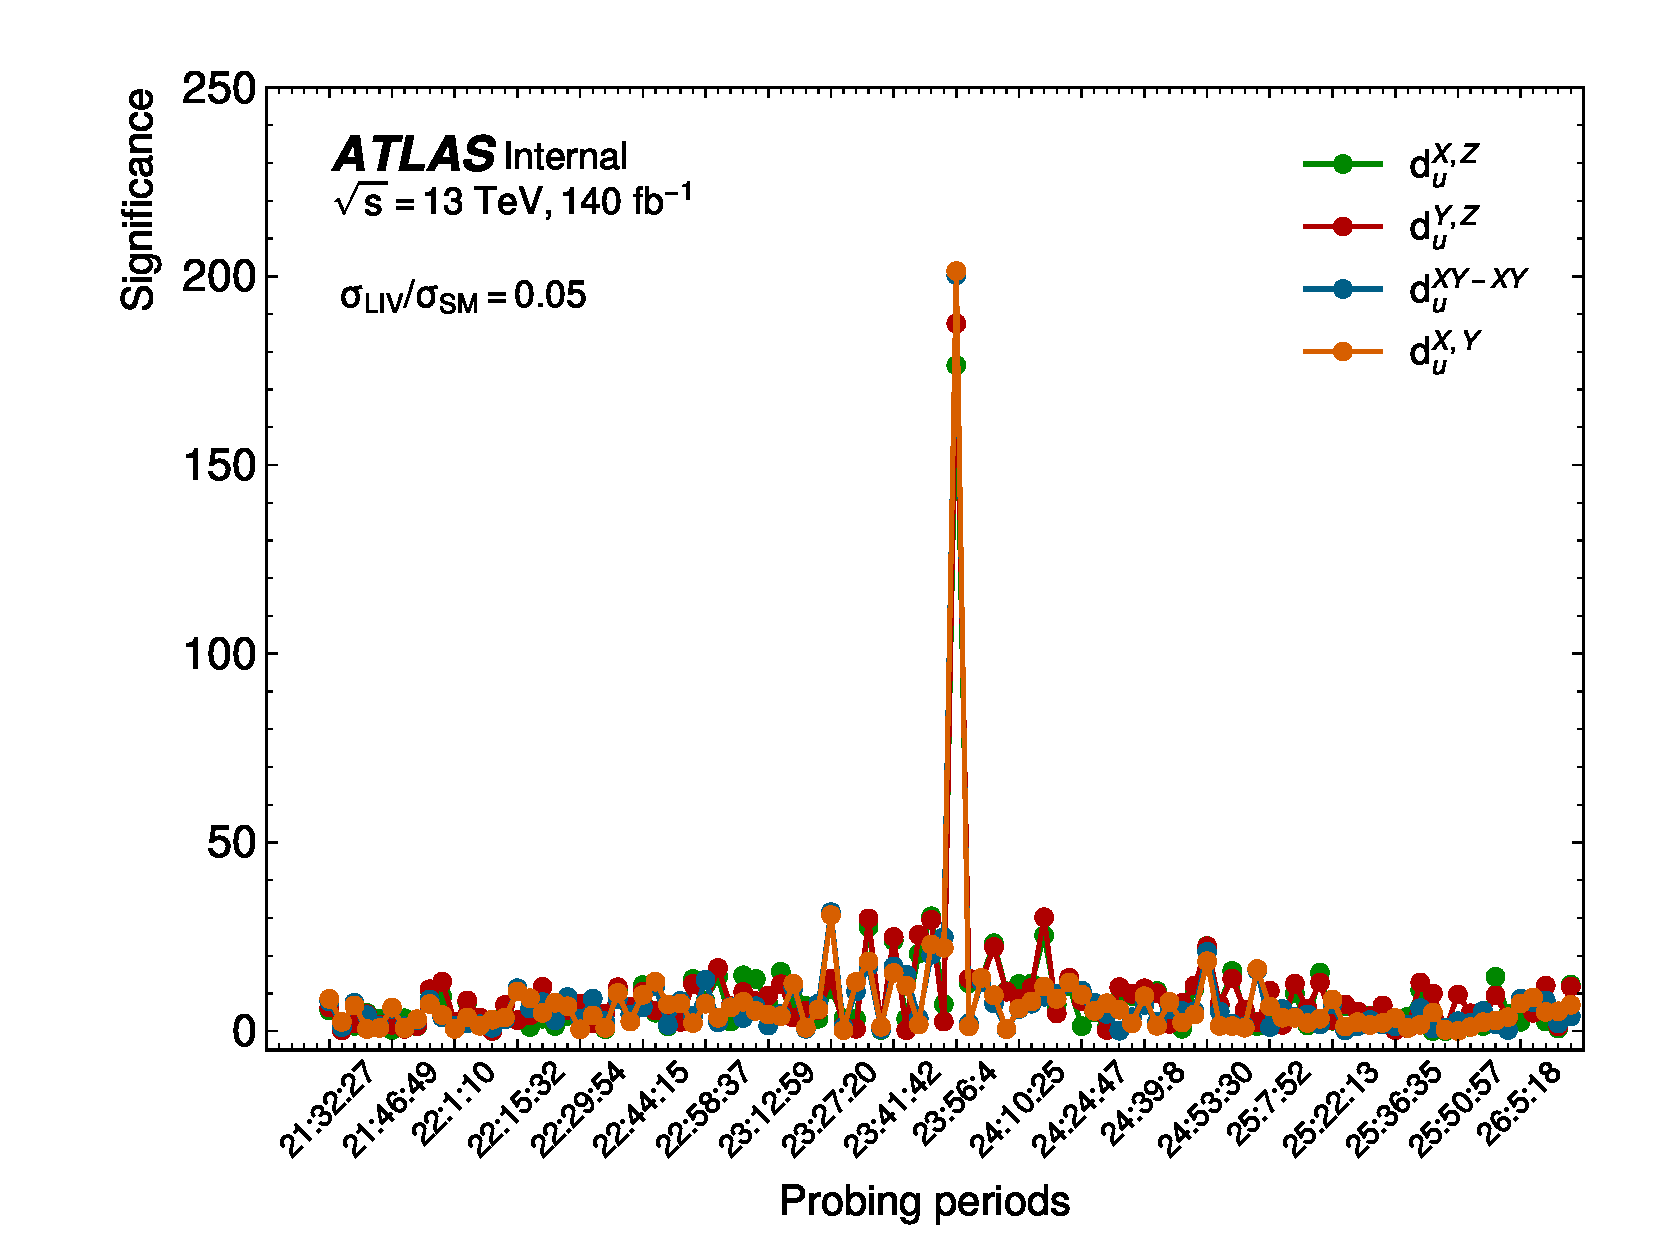
\includegraphics[width=0.45\textwidth]{figs/partially_unblinded_results/scan_periods/scan_significance_toys_with_Sys}\\
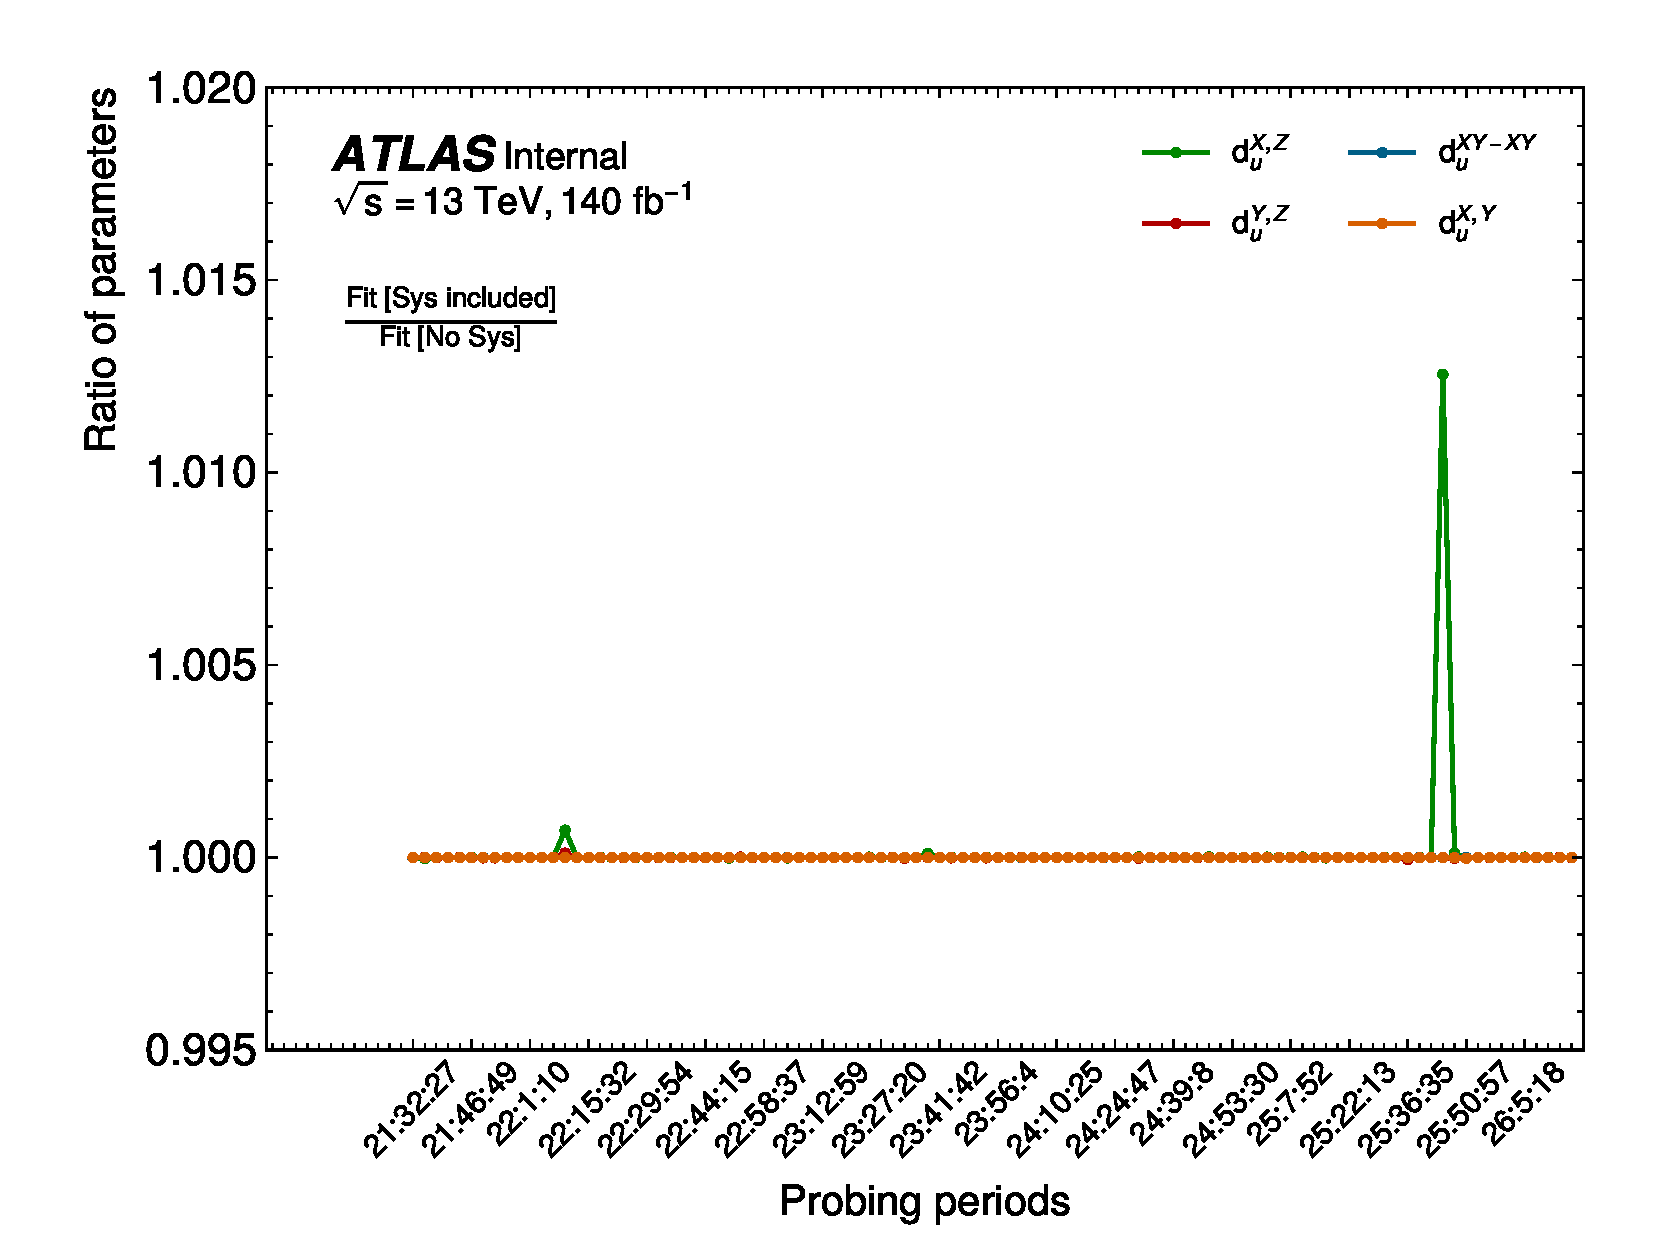
\includegraphics[width=0.45\textwidth]{figs/partially_unblinded_results/scan_periods/scan_significance_toys_Ratio_of_Fits}
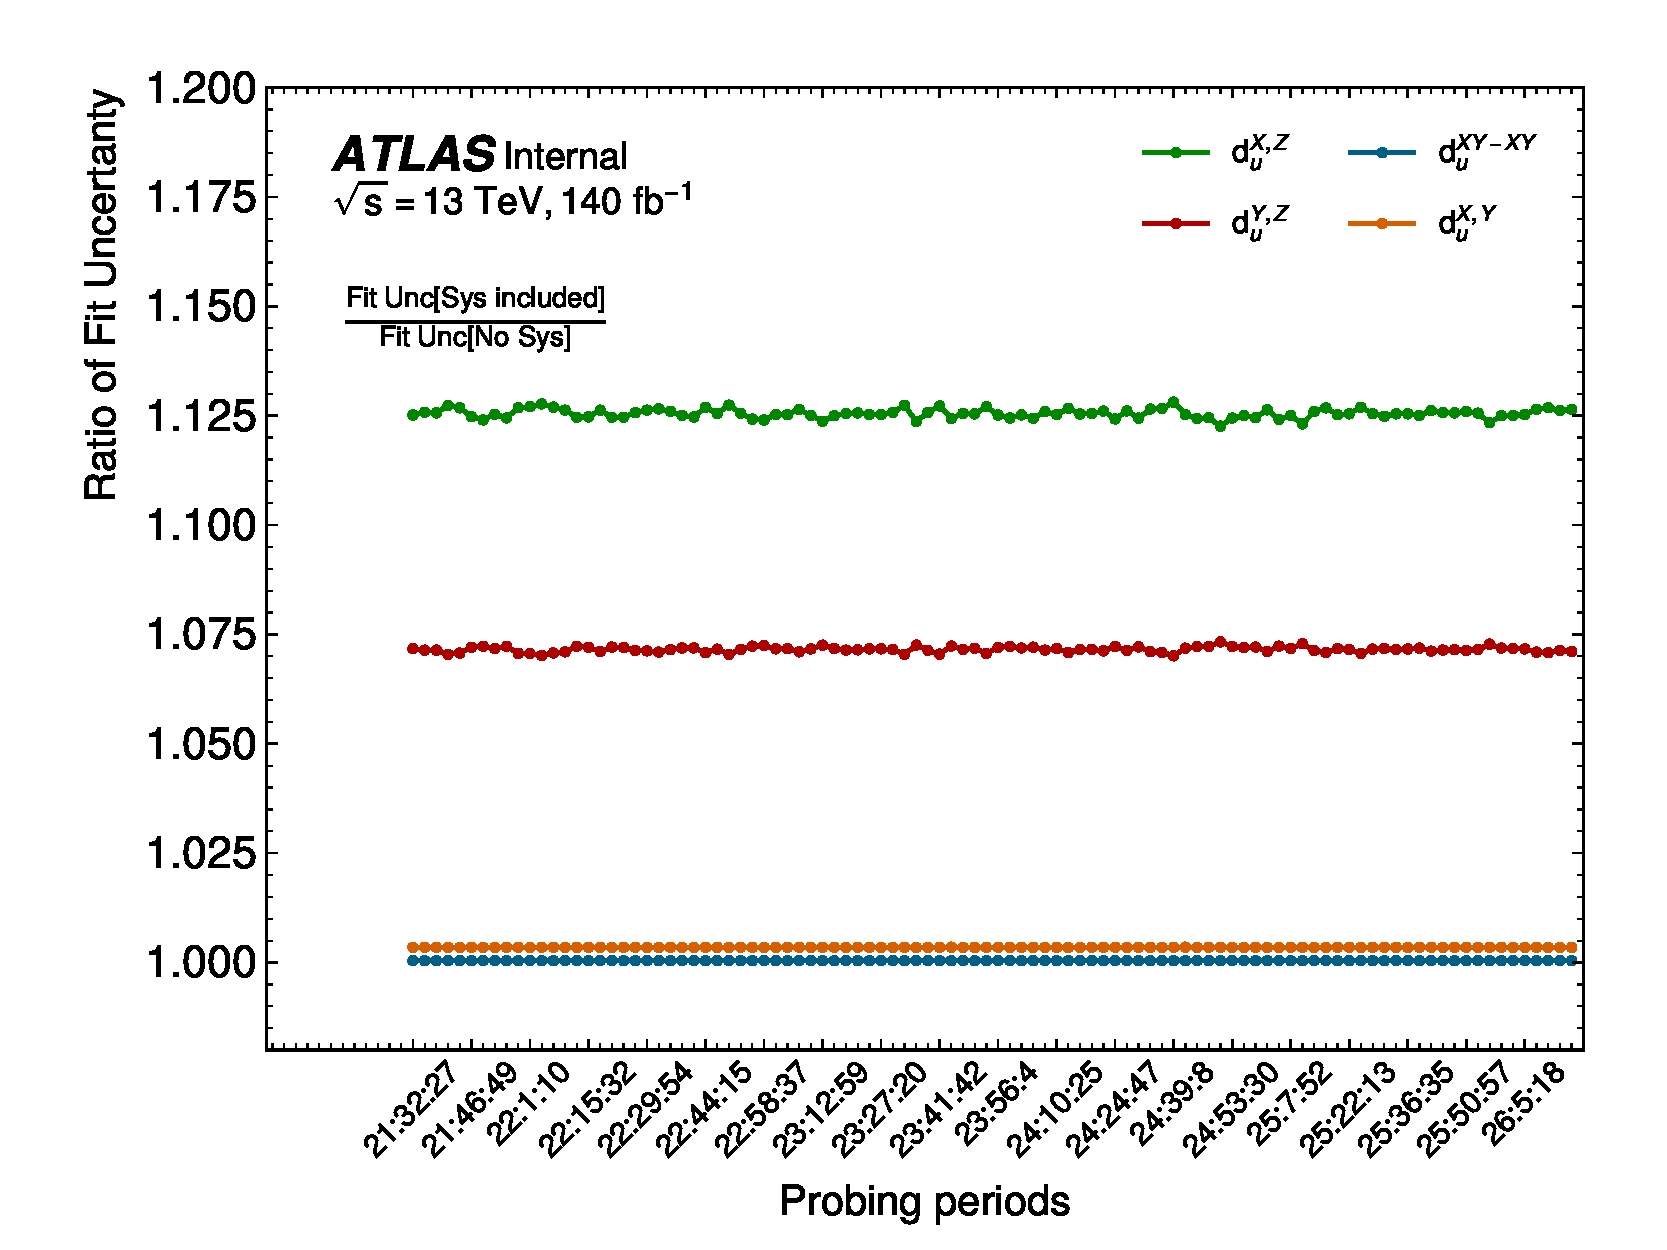
\includegraphics[width=0.45\textwidth]{figs/partially_unblinded_results/scan_periods/scan_significance_toys_impact_of_Sys}
\caption{Scan probing periods on the signal-injected toys. Four types of SME signal shapes are injected at maximum amplitude 5\% level, as shown in the plots. The top left plot shows significance without systematic is included in the fit. The Top right plot shows significance with systematic included in the fit. The bottom left plot shows the ratio of fitted parameters with/without systematic included in the fit. The bottom right plot shows the ratio of the fit uncertainties with/without systematic inclusion in the fit.}
\label{fig:scan_period_toy_Sys_combined_fit}
\end{figure}